%%%%%%%%%%%%%%%%%%%%%%%%%%%%%%%%%%%%%%%%%
% fphw Assignment
% LaTeX Template
% Version 1.0 (27/04/2019)
%
% This template originates from:
% https://www.LaTeXTemplates.com
%
% Authors:
% Class by Felipe Portales-Oliva (f.portales.oliva@gmail.com) with template 
% content and modifications by Vel (vel@LaTeXTemplates.com)
%
% Template (this file) License:
% CC BY-NC-SA 3.0 (http://creativecommons.org/licenses/by-nc-sa/3.0/)
%
%%%%%%%%%%%%%%%%%%%%%%%%%%%%%%%%%%%%%%%%%

%----------------------------------------------------------------------------------------
%	PACKAGES AND OTHER DOCUMENT CONFIGURATIONS
%----------------------------------------------------------------------------------------

\documentclass[
	12pt, % Default font size, values between 10pt-12pt are allowed
	%letterpaper, % Uncomment for US letter paper size
	%spanish, % Uncomment for Spanish
	german, % Uncomment for German
]{fphw}

% Template-specific packages

%encoding
%--------------------------------------
\usepackage[utf8]{inputenc}
\usepackage[T1]{fontenc}
%--------------------------------------
 
%German-specific commands
%--------------------------------------
\usepackage[ngerman]{babel}
\usepackage{csquotes}

\usepackage{mathpazo} % Use the Palatino font

\usepackage{graphicx} % Required for including images

\usepackage{booktabs} % Required for better horizontal rules in tables

\usepackage{listings} % Required for insertion of code

\usepackage{enumerate} % To modify the enumerate environment

%----------------------------------------
% Custom commands
\newcommand{\keyword}[1]{\textbf{#1}}

%----------------------------------------------------------------------------------------
%	ASSIGNMENT INFORMATION
%----------------------------------------------------------------------------------------

\title{Unendlichkeit und Diagonalisierungsmethode} % Assignment title

\author{Alexandra Maximova} % Student name

\date{01.04.2020} % Due date

\institute{ETH Zurich \\ Lehrdiplom Informatik} % Institute or school name

\class{Fachdidaktik 2 (Berechenbarkeit)} % Course or class name

\professor{Giovanni Serafini, Juraj Hromkovič} % Professor or teacher in charge of the assignment

%----------------------------------------------------------------------------------------

\begin{document}

\maketitle % Output the assignment title, created automatically using the information in the custom commands above

%----------------------------------------------------------------------------------------
%	ASSIGNMENT CONTENT
%----------------------------------------------------------------------------------------

\section*{Diagonalisierung und die Mächtigkeit von \(\mathbb{R}\)}

\begin{center}
	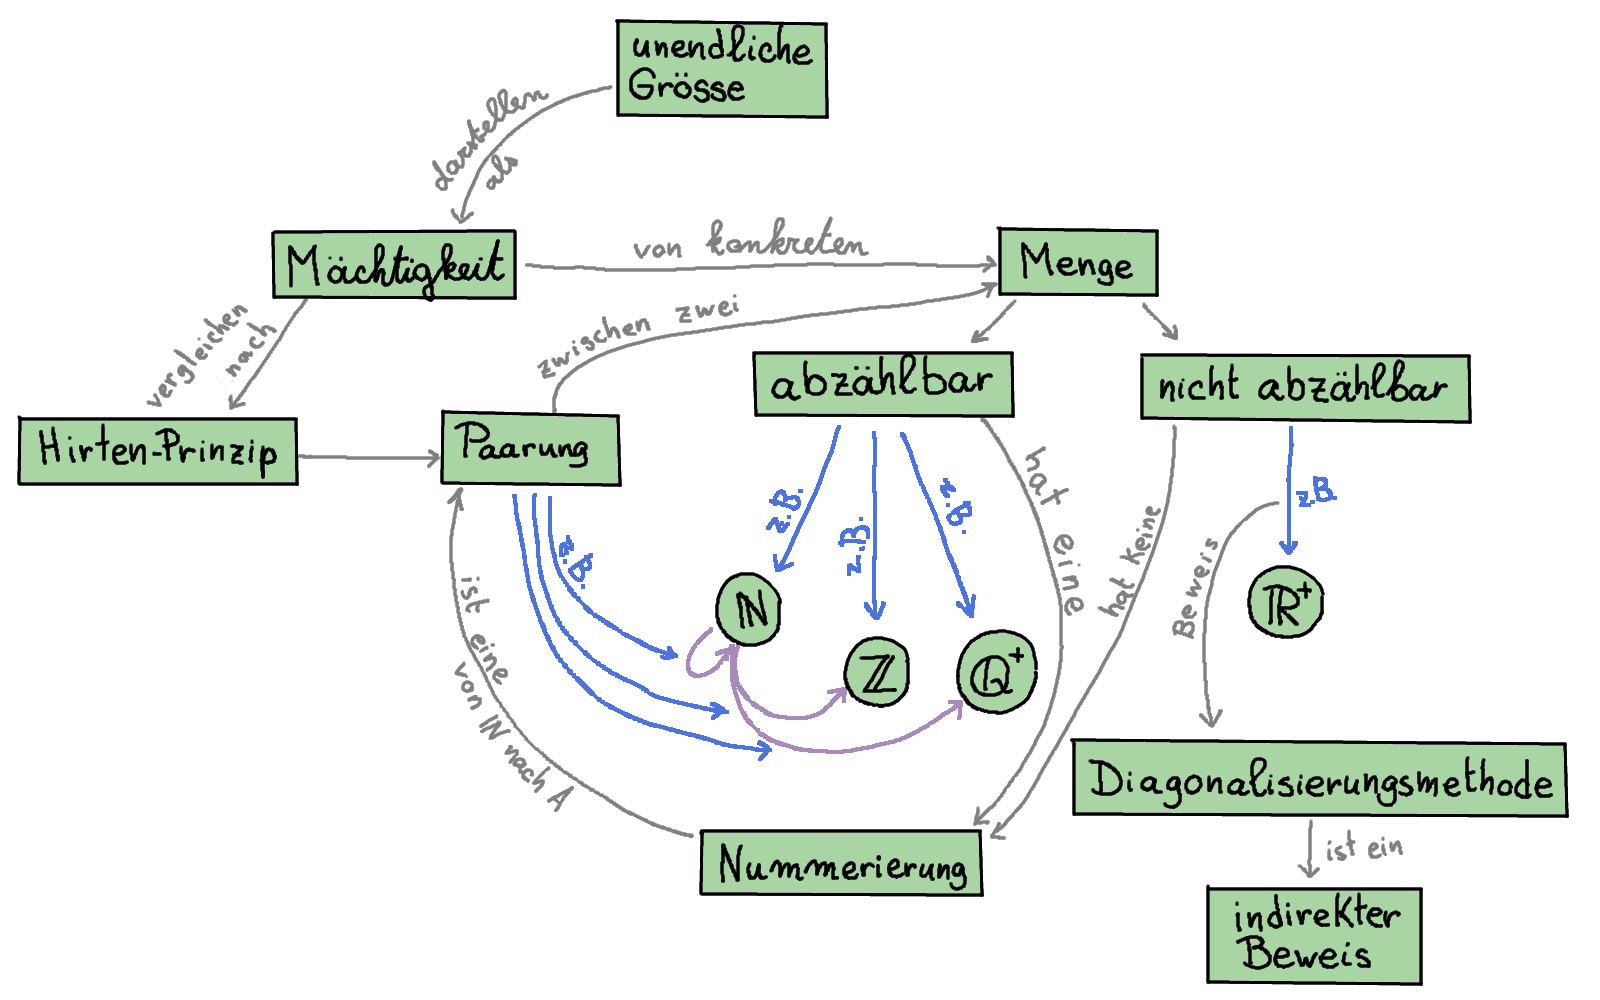
\includegraphics[width=\linewidth]{ConceptMap.png} % Example image
\end{center}


Gibt es nur einen Unendlichen? In dieser Lektion erfahren wir, dass es mindestens zwei unterschiedliche Unendliche gibt.

Eine \keyword{unendliche Grösse} wird als \keyword{Mächtigkeit} von konkreten \keyword{Mengen} dargestellt. Genau so gut wie wir die Zahl 2 als Mächtigkeit der Menge \(\{\bowtie, \bigcirc\}\) darstellen können, können wir auch Unendlich als die Mächtigkeit von zum Beispiel \(\mathbb{N}\) darstellen.

Wir können die Mächtigkeiten zweier Mengen nach dem \keyword{''Hirten-Prinzip''} vergleichen. Dies bezieht sich auf die Geschichte von einem Hirten, der nicht zählen konnte, aber wissen wollte, ob er mehr schwarze oder mehr weisse Schafe in der Herde hatte. Er hat die Herde in ''schwarzes Schaf + weisses Schaf''-Paare aufgeteilt und so die Mächtigkeit der Menge der weissen Schafe mit der Mächtigkeit der Menge der schwarzen Schafe verglichen. Genau nach diesem Prinzip nennt man zwei (auch unendliche) Mengen gleichmächtig, wenn es eine \keyword{Paarung} zwischen den Mengen gibt, d.h. es ist möglich jedem Element aus der ersten Menge ein eindeutiges Element aus der zweiten Menge zuzuordnen, und zwar so, dass in beiden Mengen kein Element alleine bleibt.

Wir haben gesehen, dass es zwischen \(\mathbb{N}\) und vielen Mengen eine Paarung hat. Eine Paarung zwischen \(\mathbb{N}\) und einer anderen Menge \(A\) nennt man eine \keyword{Nummerierung} von \(A\). Mengen, die eine Nummerierung haben, nennt man \keyword{abzählbar}. Beispiele dafür sind \(\mathbb{N}\), \(\mathbb{Z}\) und \(\mathbb{Q^+}\).

Nicht alle Mengen sind abzählbar. Zum Beispiel, in dieser Lektion konnten wir mit der \keyword{Diagonalisierungsmethode} zeigen, dass \([0,1]\), und somit auch \(\mathbb{R^+}\), keine Nummerierung haben kann und ist also \keyword{nicht abzählbar}.

Die Diagonalisierungsmethode ist ein \keyword{indirekter Beweis}. Man startet mit der Annahme, dass es eine Nummerierung gibt, und konstruiert daraus eine reelle Zahl, die nicht durchnummeriert worden ist. Das widerspricht der Annahme, deswegen muss diese falsch sein.

Daraus folgt, dass es mindestens zwei unterschiedlich grosse Unendlichen gibt: das Unendliche, welches durch \(|\mathbb{N}|\) dargestellt wird, und das Unendliche, welches durch \(|\mathbb{R}|\) dargestellt werden kann.

\end{document}
